\chapter{Matter Waves}
\chapterprecis{Louis de Broglie}

\makeoddhead{myheadings}{\emph{de Broglie}}{}{\thepage}
\makeevenhead{myheadings}{\thepage}{}{\emph{Matter Waves}}

\renewcommand{\theequation}{\arabic{equation}}

\section*{A. Phase Waves Guiding Particles}

In order to elucidate spectral phenomena, Bohr found himself forced to
relinquish, on the atomic scale, at least, a classical law of
electromagnetism: that a revolving, and hence continuously accelerating,
charge must radiate energy continuously. But Newton's laws still
functioned within Bohr's system, just as they had in Rutherford's
nuclear model of the atom. Nevertheless, a failure of electrodynamics in
the atomic microcosm laid open the question how far other macrocosmic
principles could be trusted to apply at scales of magnitude beneath the
reach of our senses. Moreover, Bohr's theory ran into ever greater
difficulties in describing the atoms of elements other than
hydrogen---atoms which must contain several electrons to remain
electrically neutral.

In contrast to mechanics, the science of optics was early forced to
acknowledge the importance of size in determining the validity of its
laws. Under ordinary conditions light travels in straight lines, or
rays, just as do particles in free space; but when it is confined to
narrow openings light spreads out into the peculiar pattern of
diffraction that indicates the presence of waves. Such waves which had
been predicted for light by Huygens and Young, were predicted also for
\emph{matter} by Louis de Broglie\footnote{The pronunciation ``de Broy''
  was attested to by Br. Robert Smith, who knew one of de Broglie's
  students.} in 1923. He reasoned that there could not be one physics
for light and another physics for matter; and that in order for the two
domains to be brought into relation with one another there had to be a
wave-particle duality for matter such as was by then already
acknowledged in the case of light. Here is de Broglie's account of the
point of departure for his hypothesis:


\section*{The Undulatory Aspects of the Electron\footnote{{[}Nobel Prize Address,
  Stockholm, 1929, from \emph{The World of the Atom}, Vol. II (New York:
  Basic Books, 1966). For the sake of consistency throughout this and
  the following chapters, the letters used by de Broglie in his
  equations have occasionally been changed.{]}}}
\begin{center}
\textbf{Prince Louis V. de Broglie}
\end{center}

\begin{quotation}
When, in 1920, I resumed my investigations in theoretical Physics after
a long interruption through circumstances out of my own control, I was
far from imagining that this research would within a few years be
rewarded by the lofty and coveted distinction given each year by the
Swedish Academy of Sciences: the Nobel Prize in Physics. At that time
what drew me towards theoretical Physics was not the hope that so high a
distinction would ever crown my labors: what attracted me was the
mystery which was coming to envelop more and more deeply the structure
of Matter and of radiation in proportion as the strange concept of the
quantum, introduced by Planck about 1900 during his researches on black
body radiation, came to extend over the entire field of Physics.

But to explain the way in which my research came to develop I must first
outline the critical period through which Physics had for the last
twenty years been passing.

Physicists had for long been wondering whether Light did not consist of
minute corpuscles in rapid motion, an idea going back to the
philosophers of antiquity, and sustained in the eighteenth century by
Newton. After interference phenomena had been discovered by Thomas
Young, however, and Augustin Fresnel had completed his important
investigation, the assumption that Light had a granular structure was
entirely disregarded, and the Wave Theory was unanimously adopted. In
this way physicists of last century came to abandon completely the idea
that Light had an atomic structure. But the Atomic Theory, being thus
banished from optics, began to achieve great success, not only in
Chemistry, where it provided a simple explanation of the laws of
definite proportions, but also in pure Physics, where it enabled a fair
number of the properties of solids, liquids and gases to be interpreted.
Among other things it allowed the great kinetic theory of gases to be
formulated, which, in the generalized form of statistical Mechanics, has
enabled clear significance to be given to the abstract concepts of
thermodynamics. We have seen how decisive evidence in favor of the
atomic structure of electricity was also provided by experiments. Thanks
to Sir J.\ J.\ Thomson, the notion of the corpuscle of electricity was
introduced; and the way in which H.\ A.\ Lorentz has exploited this idea
in his electron Theory is well known.

Some thirty years ago, then, Physics was divided into two camps. On the
one hand there was the Physics of Matter, based on the concepts of
corpuscles and atoms which were assumed to obey the classical laws of
Newtonian Mechanics; on the other hand there was the Physics of
radiation, based on the idea of wave propagation in a hypothetical
continuous medium: the ether of Light and of electromagnetism. But these
two systems of Physics could not remain alien to each other: an
amalgamation had to be effected; and this was done by means of a theory
of the exchange of energy between Matter and radiation. It was at this
point, however, that the difficulties began; for in the attempt to
render the two systems of Physics compatible with each other, incorrect
and even impossible conclusions were reached with regard to the energy
equilibrium between Matter and radiation in an enclosed and thermally
isolated region: some investigators even going so far as to say that
Matter would transfer all its energy to radiation, and hence tend
towards the temperature of absolute zero. This absurd conclusion had to
be avoided at all costs; and by a brilliant piece of intuition Planck
succeeded in doing so. Instead of assuming, as did the classical Wave
Theory, that a light-source emits its radiation continuously, he assumed
that it emits it in equal and finite quantities---in quanta. The energy
of each quantum, still further, was supposed to be proportional to the
frequency of the radiation, $\nu$, and to be equal to $h\nu$,
where $h$ is the universal constant since known as Planck's
Constant.

The success of Planck's ideas brought with it some serious consequences.
For if Light is emitted in quanta, then surely, once radiated, it ought
to have a granular structure. Consequently the existence of quanta of
radiation brings us back to the corpuscular conception of Light. On the
other hand, it can be shown---as has in fact been done by Jeans and H.\ 
Poincaré---that if the motion of the material particles in a
light-source obeyed the laws of classical Mechanics, we could never
obtain the correct Law of black body radiation---Planck's Law. It must
therefore be admitted that the older dynamics, even as modified by
Einstein's Theory of Relativity, cannot explain motion on a very minute
scale.

The existence of a corpuscular structure of Light and of other types of
radiation has been confirmed by the discovery of the photo-electric
effect which, as I have already observed, is easily explained by the
assumption that the radiation consists of quanta---$h\nu$---capable
of transferring their entire energy to an electron in the irradiated
substance; and in this way we are brought to the theory of light-quanta
which, as we have seen, was advanced in 1905 by Einstein---a theory
which amounts to a return to Newton's corpuscular hypothesis,
supplemented by the proportionality subsisting between the energy of the
corpuscles and the frequency. A number of arguments were adduced by
Einstein in support of his view, which was confirmed by Compton's
discovery in 1922 of the scattering of X-rays, a phenomenon named after
him.\footnote{{[}In 1922, Arthur Compton had demonstrated experimentally
  that, with de Broglie's assumptions, the interaction of x-rays with
  electrons can be understood as \emph{particle-like collisions} between
  electrons and photons, in which the x-ray photon transfers some of its
  energy to the electron and thus changes its own wavelength and
  momentum. His measurements showed that then both energy and momentum
  were conserved in these interactions.{]}} At the same time it still
remained necessary to retain the Wave Theory to explain the phenomena of
diffraction and interference, and no means was apparent to reconcile
this Theory with the existence of light-corpuscles.

I have pointed out that in the course of investigation some doubt had
been thrown on the validity of small-scale Mechanics. Let us imagine a
material point describing a small closed orbit---an orbit returning on
itself; then according to classical dynamics there is an infinity of
possible movements of this type in accordance with the initial
conditions, and the possible values of the energy of the moving material
point form a continuous series. Planck, on the other hand, was compelled
to assume that only certain privileged movements---quantized
motion---are possible, or at any rate stable, so that the available
values of the energy form a discontinuous series. At first this seemed a
very strange idea; soon, however, its truth had to be admitted, because
it was by its means that Planck arrived at the correct Law of black body
radiation and because its usefulness has since been proved in many other
spheres. Finally, Bohr founded his famous atomic Theory on this idea of
the quantization of atomic motion---a theory so familiar to scientists
that I will refrain from summing it up here.

Thus we see once again it had become necessary to assume two
contradictory theories of Light, in terms of waves, and of corpuscles,
respectively; while it was impossible to understand why, among the
infinite number of paths which an electron ought to be able to follow in
the atom according to classical ideas, there was only a restricted
number which it could pursue in fact. Such were the problems facing
physicists at the time when I returned to my studies. When I began to
consider these difficulties I was chiefly struck by two facts. On the
one hand the Quantum Theory of Light cannot be considered satisfactory,
since it defines the energy of a light-corpuscle by the equation
$E = h\nu$, containing the frequency $\nu$. Now a purely
corpuscular theory contains nothing that enables us to define a
frequency; for this reason alone, therefore, we are compelled, in the
case of Light, to introduce the idea of a corpuscle and that of
periodicity simultaneously. On the other hand, determination of the
stable motion of electrons in the atom introduces integers; and up to
this point the only phenomena involving integers in Physics were those
of interference and of normal modes of vibration. This fact suggested to
me the idea that electrons too could not be regarded simply as
corpuscles, but that periodicity must be assigned to them also. In this
way, then, I obtained the following general idea, in accordance with
which I pursued my investigations:---that it is necessary in the case of
Matter, as well as of radiation generally and of Light in particular, to
introduce the idea of the corpuscle and of the wave simultaneously: or
in other words, in the one case as well as in the other, we must assume
the existence of corpuscles accompanied by waves. But corpuscles and
waves cannot be independent of each other [\ldots]. It must consequently be
possible to establish a certain parallelism between the motion of a
corpuscle and the propagation of its associated wave. The first object
at which to aim, therefore, was to establish the existence of this
parallelism.

\end{quotation}

\begin{center}
* * *
\end{center}

De Broglie went on to ``establish the existence of this parallelism'' by
outlining an idea of ``matter waves'' complementary to Planck's light
quanta. If the quantum treatment of light gives to the classical light
wave an accompanying \emph{particle} (the photon), so also de Broglie
will give the classical Newtonian particle of matter an accompanying
matter \emph{wave}. Since the Planck-Einstein hypothesis makes the
photon's energy proportional to the frequency of its associated light
wave, so too will de Broglie ascribe a frequency $\nu$~ to the wave
that accompanies a material particle---a frequency related to the
particle's total energy $E$ according to the very same equation as
Planck's, $E = h\nu$. Thus to every material body endowed with
total energy $E$ de Broglie associates a corresponding wave and
ascribes to that wave a frequency given by:
\begin{equation*}
\nu\,\text{(of matter wave)} = \frac{E\,\text{(of material body)}}{h}
\end{equation*}
For the wavelength of the proposed matter wave, de Broglie similarly
carries over a relation previously established for light. Maxwell had
demonstrated that a light wave conveys momentum to the surface that
absorbs it, in the amount
\begin{equation*}
p = \frac{E}{c}
\end{equation*}
where $p$ is the momentum and $E$ is the energy delivered,
over any period of time, to the absorbing surface. By Planck's
hypothesis, each quantum of light energy $E$ may be expressed as
$E = h\nu$ , so that, substituting,
\begin{equation*}
p = \frac{h\nu}{c} = \frac{h}{\lambda};
\end{equation*}
which implies that \emph{a light quantum possesses} \emph{momentum
inversely proportional to its wavelength}. De Broglie extends this same
relation to the proposed matter wave; thus, if the material body has
momentum $p$, de Broglie ascribes to the corresponding wave a
\emph{wavelength} given by:
\begin{equation*}
\lambda\,\text{(of matter wave)} = \frac{h}{p\,\text{(of material body)}}.
\end{equation*}

Finally, de Broglie assumes that the postulated matter wave obeys the
usual relation $u = \nu\lambda$ between frequency, wavelength, and
wave velocity, so that the matter wave corresponding to a body endowed
with energy $E$ and momentum $p$ will propagate with a
\emph{velocity} given by:
\begin{equation*}
u\text{(of matter wave)}=\nu\lambda=\frac{E}{h}\cdot\frac{h}{p}=
\frac{E\,\text{(of material body)}}{p\,\text{(of material body)}}.
\end{equation*}

At first sight, this result would not appear to tell us anything
plausible about the wave speed, since for a body moving with speed
$w$ and so having kinetic energy in the amount $\frac{1}{2}mw^2$ and
momentum equal to $mw$, $u$ is equal to $\frac{1}{2}w$: the wave
travels with half the speed of the particle! But de Broglie points out
that the energy $E$ in the above expressions is the \emph{total}
energy of the body---and according to relativity theory, a body's
kinetic energy represents only a tiny part of its total energy, unless
that body moves with speeds comparable to that of light! We will derive
this astonishing result in the second-semester senior mathematics
tutorial. De Broglie accepts it as given, and on that basis
assumes---remember, he \emph{only} assumes---that the wave velocity
$u$ is inversely proportional to the particle speed $w$:
$wu = c^2$, where $c$ is the speed of light in empty
space.\footnote{Here are the grounds for the assumption. The
  relativistic \emph{mass-energy equivalence theorem} holds that a
  body's mass $m$ represents a contribution, called the body's
  \emph{rest energy}, of $E_{\text{rest}} = mc^2$ to its total energy
  ($c$ being the speed of light); thus, since $c$ is very
  large, it is clear that for any realistic speeds, a body's total
  energy will scarcely exceed this rest energy. Then, in the earlier
  expression for the velocity of the matter wave, we have $u =
  E_{\text{total}}/p \approx mc^2/mw$ or $uw \approx c^2$.

  Note that henceforth we shall continue to use $w$, instead of
  $v$, to refer to the speed of a particle. This is done in order
  that the reader not mistake the speed for the frequency $\nu$.}

De Broglie's new, postulated, wave is not a wave in the electromagnetic
field and does not itself carry energy; nevertheless it is conceived as
governing the motion of the particle. At this stage of trying to
conceive of ways in which the matter waves and the material particle
might be related, de Broglie proposes the metaphor of guiding; the waves
might ``guide'' the particle. If a body's motion corresponds to this
\emph{guiding wave} in the same way that a ray of light is determined by
the self-coherent interference pattern of light waves spreading
throughout all space, then---de Broglie argues---there is a possibility
of explaining why the electron in the hydrogen atom is able to move only
in those discrete orbits, discontinuous from one another, that Bohr
discovered.

But how \emph{could} such a wave guide a particle? In a later article,
in which he reflects on his papers of 1923 and his dissertation of 1924,
de Broglie writes:

\begin{quotation}
I was seeking to picture to myself a real physical wave carrying a very
small localized object in space through the passage of time. Two ways of
doing so then presented themselves to my mind. The first, [\ldots] which I
now consider to be much more profound, was [\ldots] developed in the first
chapter of my dissertation. It consisted in beginning with the
difference in the relativistic transformations of the frequency of a
wave and of the frequency of a clock. Admitting that the particle
possesses an internal vibration which permits its being likened to a
little clock, I supposed that this clock displaced itself in its wave in
such a way that its internal vibration remains constantly in phase with
that of the wave: this is the postulate of ``the agreement of phases.''
These hypotheses appeared to me to be made necessary by the fact that
the relation $E = h\nu$, applied to the particle, implies the
existence of a frequency $\nu$ internal to the particle, whereas,
since the works of Planck and Einstein, it is known that $\nu$ is
\emph{also} the frequency of the wave that carries the particle. The
particle appears then as incorporated into the wave in which it
constitutes a very small region where the amplitude is very large. From
this one can deduce the [\ldots] formula $p =h/\lambda$.\footnote{``Sur 
  les véritables idées de base de la
  mécanique ondulatoire'' in \emph{Recherches d'un demi-siècle} (Paris:
  Albin Michel, 1976), 64.

  De Broglie went on to develop the second way: ``In the second chapter
  of my dissertation, I then had shown that, \emph{in the case where the
  wave propagation takes place approximately as in geometrical optics},
  we are led to identify Fermat's principle {[}of least time in
  optics{]} with Maupertuis's principle of least action {[}in
  mechanics{]}'' (italics added). His reasons for preferring the first
  way were that, of the two, only it is ``essentially relativistic'' in
  the sense of special relativity and holds even for wave propagations
  that are \emph{not} approximately the same as those in geometrical
  optics. In Section C we shall return to the approximate character of
  geometrical optics in de Broglie's view.

  In spite of the possible advantages of the first way, it was by
  pursuing the second way that Schrödinger was able to determine the
  differential equation for the matter waves. For a discussion of the
  principles of Fermat and Maupertuis, see the introduction to
  Schrödinger's paper in Chapter 10.}
\end{quotation}

If every portion of matter is thought of as containing some sort of
internal vibration or oscillation,\footnote{Whereas here the frequency
  of oscillation varies as the energy of the particle, in Planck's
  analogy the frequency of each oscillator was fixed and determined the
  size of the packets of energy that an oscillator could hold, absorb,
  or radiate.} then the particle and its associated wave may be brought
into connection through their common property of frequency. This, he
states, implies a criterion by which the associated wave can
\emph{distinguish one path from another}, and so play a guiding role for
the particle. ``Agreement of phases'' seems to mean that, when the
``hand'' on the body's internal clock has swept out some part of a
complete revolution, it will be at that instant at a point in space at
which its guiding wave is in exactly the same phase of its cycle. This
leads de Broglie to call the wave associated with the particle its
\emph{phase wave}. The particle carries energy, but the wave
``carries'' the particle, \emph{guiding it} \emph{through the only
trajectory that keeps the two in phase}. Thus agreement of phases
between particle and associated wave is the sought-for criterion that
distinguishes the particle's actual path from other, hypothetical,
paths.

A second consequence of de Broglie's assumptions is to secure formal
agreement between optical laws governing motion of light rays and
dynamical laws that determine the motion of particles---and ultimately,
the ``synthesis'' of waves and particles:

\begin{quotation}
{[}I.{]} We propose to base the dynamics of material particles on the
following postulate: In each point of its trajectory, a freely moving
particle follows with a uniform motion the \emph{ray} of its phase wave,
that is, (in an isotropic medium) the normal to the surfaces of equal
phase [\ldots].

This new principle on which dynamics is to be based would explain the
diffraction of light quanta, \emph{however small their number}.
Moreover, \emph{any} moving particle would be subject to diffraction
given the appropriate circumstances. A flow of electrons, for example,
passing through a sufficiently small slit, would be expected to show
diffraction phenomena. It is from this direction that experimental
confirmation of our ideas will perhaps have to be sought.\footnote{{[}Diffraction
  of electrons was observed experimentally only four years after de
  Broglie's proposal.{]}}

Hence we conceive the phase wave as guiding the displacements of energy,
and this is what enables the synthesis of waves and quanta. The wave
theory went too far when it denied the discontinuous structure of
radiant energy and not far enough when it refused to intervene in
dynamics. \emph{The new dynamics of the free material particle is to
the old dynamics [\ldots] what wave optics is to geometrical
optics.}\footnote{{[}Or what Young's optics (\emph{Mechanics}, 159ff.)
  is to Newton's optics (\emph{ibid}., 149ff.).{]}} In reflecting on it
one will see that the proposed synthesis of waves and quanta is the
logical coronation of the comparative development of dynamics and optics
since the 17th century.

{[}II.{]} Let us come now to the explanation of interference bands. Let
us suppose that a material atom has a probability of absorbing or
emitting an atom of light that is determined by {[}the square of the
amplitude{]} of one of the phase waves that cross each other in passing
over it. Of course, emission is possible only if the {[}material{]} atom
is excited, while absorption is possible only if a light atom is present
nearby. The preceding hypothesis is completely analogous to that of the
electromagnetic theory when that theory connects the \emph{detectable}
intensity of light [\ldots] with the intensity of the electric field
vector.\footnote{[At the end of Junior Laboratory, Maxwell's argument
  that light is an electromagnetic wave was studied. Earlier the energy
  density (energy per unit volume) in an electromagnetic field had been
  shown to be proportional to the square of the field strength, here
  represented by $F$: $E/V \propto F^2$. The
  \emph{intensity} of a wave ($I$) is defined as the amount of
  energy ($E$) that flows per second ($t$) across unit area
  perpendicular to the direction of travel ($A$). Hence, if
  $s$ represents distance in the direction of travel, then
  \begin{equation*}
  I \equiv \frac{E}{tA} = \frac{Es}{tAs} = \frac{E}{As}\frac{s}{t} =
    \frac{E}{Vol}c \propto F^2 ,
  \end{equation*}
  where $c$ is the speed of light. Or since both $I$ and
  $F$ are different at different places and times:
  $I(x,y,z,t) \propto F(x,y,z,t)^2$. Thus, the
  intensity of light is proportional to the square of the amplitude of
  the electric field vector.

  On the other hand, the Einstein reading in Chapter 6 showed that the
  intensity of light is proportional to the number of photons ($N$)
  passing per second through a unit area perpendicular to the direction
  of travel. If the time interval is small enough, then $N$ will be
  less than one. Since a photon is not divisible, we could regard
  $N$ as a measure of the probability ($P$) that a photon will
  pass through $A$ as was done with alpha particles in the
  introduction to the chapter on Rutherford. Thus, $P(x,y,z,t) \propto N \propto I \propto
  F(x,y,z,t)^2$. Hence, the probability that an
  electric field will manifest itself as a particle, a photon, in a
  given area is also proportional to the square of the amplitude of the
  electric field vector. De Broglie refers to this in the second
  sentence of the paragraph.]}

When any cause whatever has triggered the emission of a light quantum in
a ``point'' source, its phase wave, in traversing the neighboring atoms,
will trigger other emissions of light quanta, the internal vibration of
which we shall suppose in phase with the wave itself.\footnote{{[}De
  Broglie has thus interpreted Maxwell's electromagnetic waves as being
  guiding waves, which guide light quanta in the same way as de
  Broglie's matter waves guide material particles.{]}} Therefore, all
the emitted light quanta will have the same phase wave as the first
quantum. We shall say that they are `phase-coupled'. Thus, a single
phase wave {[}of light{]} carries along with itself a throng
{[}\emph{une foule}{]} of little bits of energy [\ldots].

Let us consider then Young's double-slit experiment.\footnote{{[}\emph{Mechanics},
  167ff.{]}} Some light quanta pass through the slits; and they will be
diffracted because {[}according to our theory{]} they must follow the
\emph{ray} of the phase wave in their vicinity. In the spaces beyond the
double slit, their capacity to act photoelectrically {[}i.e., to be
absorbed by an electron{]} will vary at each point, according to the
state of interference of the phase waves which have been diffracted by
the two slits. Hence, \emph{however weak the intensity of the incident
light may be}, there will be bright and dark bands such as had been
predicted by the wave theories.

This mode of explanation, which borrows its essential points from wave
theory in the very act of introducing quanta, is to be generalized so as
to deal with all interference and diffraction phenomena.\footnote{``Quanta
  de Lumière, Diffraction et Interférences,'' \emph{Comptes rendus} 177
  (1923), 548, in \emph{Recherches d'un demi-siècle} (Paris: Albin
  Michel, 1976).}
\end{quotation}

\emph{Light Waves and Einstein's Photons.} As we have seen, de
Broglie's discussion of light above supplements Einstein's quantum
hypothesis by interpreting the Maxwellian wave as guiding photons
analogously to the way in which matter waves guide electrons.

Consider monochromatic diffracted light falling on a screen. De Broglie
postulates that at any point on the screen the probability of a photon
interacting with an atom (or an electron) there is directly proportional
to the square of the amplitude of the Maxwellian wave there. This
implies that \emph{the number of such interactions per second} at
different regions on the screen is proportional to the squared amplitude
of the waves hitting those points. And each interaction delivers one
quantum of energy, so that the measurable intensities, that is, the
energy delivered per second per unit area, are naturally proportional to
the same thing.

Furthermore, consider \emph{one photon} going through a slit. The
relative probability that it will eventually interact with an atom at
one point on the screen compared with another is in this hypothesis
proportional to the squared amplitude of the Maxwellian wave at those
points.

\section*{B. Refraction of Matter Waves: Application to the Orbiting
Electron }

De Broglie applied the mode of explanation outlined in the previous
quotation to the phenomenon of refraction that would have to be involved
in the case of the orbital electron of the hydrogen atom.

\begin{quote}
The most interesting application is the study of the atom of hydrogen as
conceived by Bohr. We now regard the atom of hydrogen as a refracting
sphere, which, for the waves accompanying the motion of an electron of
charge, $e$, possesses a refractive index\footnote{{[}Huygens had
  shown that his wave theory of light implied that the ratio of the sine
  of the angle of incidence to the sine of the angle of refraction was
  the same as the ratio of the speeds of the waves in the two media
  (\emph{Treatise on Light}, \emph{Mechanics,} 123ff.), or,
  written in terms of fractions: $\sin\theta_i/\sin\theta_r = c_i/c_r$, where
  $c_i$ and $c_r$ refer to the
  speeds of light in the incident and refracting media, respectively.
  The number $n = \sin\theta_i/\sin\theta_r = c_i/c_r$ is the \emph{index
  of refraction} of medium $r$ with respect to medium $i$, and this equation
  is known as \emph{Snell's Law}. The index of refraction of a vacuum,
  where the speed of light is $c$, is taken to be 1. If the vacuum
  is taken as a standard, an index of refraction,
  $n_{med}$, can be assigned to any medium:
  $n_{med} = c/c_{med}$.{]}}
which varies {[}from point to point\ldots]. The rays which return into
themselves coincide with the possible trajectories of the electron, and
some of them possess the very remarkable property of being in resonance
with the wave: it is just these rays which are the ``stable''
trajectories of Bohr.\footnote{{[}L. de Broglie, ``On the Parallelism
  between the Dynamics of a Material Particle and Geometrical Optics,''
  14 in \emph{Selected Papers on Wave Mechanics} (London: Blackie \&
  Sons, 1928), originally published in \emph{Journal de Physique} 7
  (1926).{]}}
\end{quote}

In two different ways the refraction involved here is more complicated
than that discussed in the \emph{Mechanics} manual. First, whereas
Huygens studied refraction at the boundary of two surfaces of noticeably
different indices of refraction, the refraction of the matter waves
around the hydrogen orbits would be analogous to light waves' being bent
in a \emph{gradual curve} due to the medium's being made of
non-uniform glass such that the glass's index of refraction
\emph{varied continuously} from point to point. Then the index of
refraction $n$ would depend on the location within the glass:
$n = n(x,y,z)$. For the case of a spherical orbit, de
Broglie considers ``a medium with spherical symmetry in which the
refractive index varies {[}inversely{]} with the distance $r$ from
the centre,''\footnote{\emph{Ibid}., 13-14.} so that $n \propto 1/r$.

\begin{wrapfigure}[18]{R}{0.4\textwidth} % Figure 1
  \begin{center}
    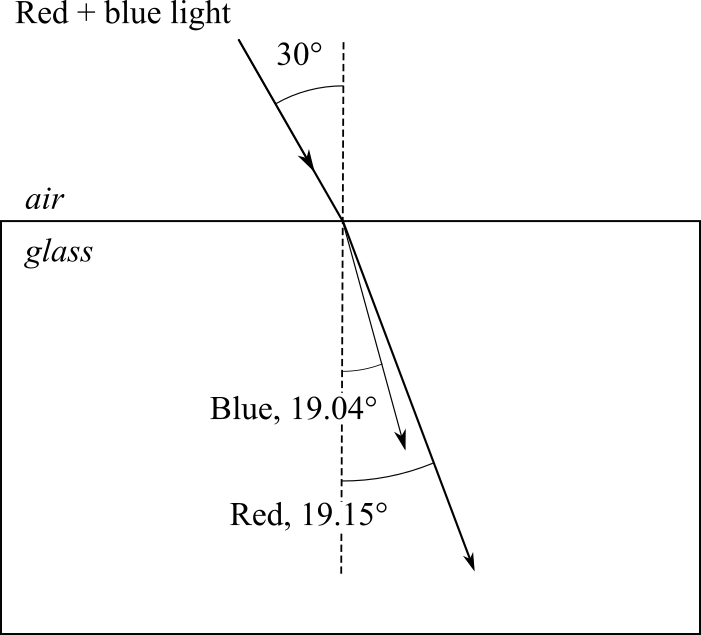
\includegraphics[width=2.338in,height=2.117in]{images/08_debroglie/refraction.png}
    \caption*{\emph{Figure 1: Light beams of different wave-lengths refract at different
    angles in a dispersive medium. (The angular difference is exaggerated in
    this drawing.)}}
  \end{center}
\end{wrapfigure}


Second, Newton had shown that the ``Analogy between colors and
refrangibility is very strict, the Rays always either exactly agreeing
in both or proportionally disagreeing in both'' (\emph{Mechanics}, 
154). In the wave theory of light, the property of the wave that is
constant when the wave passes from one medium to another is its
frequency, while its speed and wavelength both change. Thus, light of
different frequencies is refracted in different amounts in the same
medium, that is, the index of refraction of light depends on its
frequency.



Whenever the separate colors in white light spread out into a spectrum
upon passing through a prism, it is because waves of different
frequencies are being propagated at different speeds, causing their rays
to bend along different paths. For example, when red light of wavelength
6563 Å shines on the flat surface of a piece of crown glass at an angle
of incidence of 30$^{\circ}$, it will be refracted within the glass at an angle
of 19.15$^{\circ}$ (Fig. 1). By Snell's law, the sines of these angles will be in
the same ratio as the speeds of the light in the air and in the glass,
respectively. The frequency remains the same, so the wavelength must
diminish in the glass, in the same ratio in which the speed is reduced.
Thus,
\begin{equation*}
n^{red} = c^{red}_{air}/c^{red}_{glass}=\sin 30^{\circ}/\sin 19.15^{\circ}
= \lambda^{red}_{air}/\lambda^{red}_{glass}.
\end{equation*}

The speed of light in air, virtually the same as in vacuum, is about
186,000 miles/sec or $3\!\times\!10^{8}$ m/sec---denoted by the letter $c$.
Then, knowing the wavelength of this red light in air, we may calculate
its speed and wavelength in the glass. Similarly, blue light of
wavelength 4861 Å entering the same glass at the same angle will refract
at 19.04$^{\circ}$. At what speed then does this blue light travel in the glass
and what is its index of refraction?

In describing ``the manner how colors are produced by the Prism,''
Newton wrote that ``the Rays [\ldots] by their unequal refractions must be
severed and \emph{dispersed} into an oblong form in an orderly
succession from the least refracted Scarlet to the most refracted
Violet'' (\emph{Mechanics}, 156; italics added). The prism is said to
be a \emph{dispersive medium}, and the phenomenon of spreading-out is
called \emph{dispersion}.

So, in dispersive media for matter waves, the index of refraction would
have to depend on the frequency of the waves, in addition to the
location: $n = n(x,y,z,\nu)$. In the particular case of
spherical symmetry: $n \propto f(\nu)/r$, where
$f$ is some function of $\nu$.

De Broglie first proved the general theorem enunciated below and then
applied it to an electron orbiting the hydrogen nucleus, understood as
analogous to light waves moving in a spherically symmetrical, dispersive
medium:

\begin{quotation}
Now let us suppose that at time $t = 0$ the moving particle
coincides in space with a wave of frequency $\nu$, which propagates
with speed $u = c^2/w$ in the same direction as the
particle. This wave of speed greater than $c$ cannot correspond to
a propagation of energy;\footnote{{[}The product of wave and particle
  speeds has been supposed equal to the speed of light squared.
  Therefore, since the particle speed is certainly less than the speed
  of light, the wave speed must be supposed \emph{greater} than the
  speed of light. But it is a tenet in relativity theory that no actual
  process can transmit energy with a speed greater than that of light;
  so the associated wave ``cannot correspond to a propagation of
  energy.'' Hence de Broglie calls it ``fictional'' above.{]}} we
consider it only as a fictional wave associated with the motion of the
moving particle.

I say that, if at time $t$ = 0 there is agreement of phase between
the {[}guiding{]} wave and the internal {[}vibrational{]} phenomenon of
the moving particle this agreement of phase will continue [\ldots].

Let us now pass to the case of an electron describing a closed
trajectory at a uniform speed considerably less than $c$. At time
$t$ = 0 the moving particle is at a point P. The associated fictive
wave, departing then from P and describing the complete closed
trajectory at {[}a constant speed much greater than that of the
electron{]}, catches up with the electron at time $\tau$ and at point
P'.\footnote{{[}``Ondes et Quanta,'' \emph{Comptes rendus} 177
  (1923), 507, in \emph{Recherches d'un demi-siècle} (Paris: Albin
  Michel, 1976). We shall not attempt to follow de Broglie's proof.{]}}
\end{quotation}

After calculating the period of revolution of the electron around its
orbit and the internal phase of the electron upon reaching point P', de
Broglie concluded:

\begin{quote}
It is \emph{almost necessary} to suppose that the trajectory of the
electron is stable \emph{only} if the fictive wave passing at P' finds
the {[}internal vibration of the{]} electron in phase with it. The wave
must be in resonance {[}with the electron's internal vibration{]} over
the length of the trajectory {[}actually followed by any orbiting
electron{]}.\footnote{{[}``Ondes et Quanta,'' \emph{Comptes
  rendus} 177 (1923), 507--508, in \emph{Recherches d'un demi-siècle}
  (Paris: Éds, Albin Michel, 1976). De Broglie's symbols have been
  changed.{]}}
\end{quote}

De Broglie then demonstrated that an equation equivalent to Bohr's
equation (8) in Chapter 7 above followed from this ``condition of
stability.'' The general idea is that the requirement of staying in
resonance with the electron's internal vibration around the orbit
restricts the fictive matter waves to a particular set of wavelengths
and also to particular distances from the nucleus, which turn out to be
the same as the radii of Bohr's orbits. By virtue of the de Broglie
relation, $\lambda = h/p$, these allowable wavelengths then
determine the electron's momentum and hence the kinetic energy,
$KE = p^2/2m$, of the system,
leading to the discrete energy values (the potential energy being
inversely proportional to the distance) that Bohr had been forced to
postulate.

For since the electron is circling around the orbit, the ray of the
fictive waves and the fictive waves themselves are also circling upon
themselves around that orbit. Hence, since, by de Broglie's condition of
stability, the internal periodic phenomenon of the electron must remain
in phase with its guiding waves; therefore, those waves, as they
continually superimpose each of their circuits on its previous ones,
\emph{must remain in phase with themselves}. This condition will be met,
however, only if the circumference of the orbit is \emph{equal to} the
de Broglie wavelength, or twice, or three times, or \emph{any}
\emph{integral multiple of the wavelength}.

But this is exactly what happens in the second, or third, or any Bohr
orbit; in general, for the $n^{\text{th}}$ Bohr orbit, the circumference
$2\pi a_n$ will equal $n\lambda_n$.\footnote{This general result is easy to show
  by adding subscripts to Eq.\ (i) of note 10 and
  Eq.\ 8 in the main text of Chapter VII. Between equations 
  $mw_n^2 = e^2/a_n$ and $2a_n = n^2h^2/2\pi^2me^2$,  eliminate $e$ to obtain
  $4\pi^2a_n^2 = n^2h^2/m^2w_n^2$. Taking
  square roots then yields $2\pi a_n = nh/mw_n$;
  but since $h/mw_n = \lambda_n$, we see
  that the orbital circumference $2\pi a_n$ is always
  an integral multiple $n$ of the electron's associated wavelength
  for that orbit.

  Thus it was for a time accepted that in-phase overlapping of the
  wavelengths is what determines the eligible orbits of a particle.
  However, this neat result proved to be valid only for hydrogen, and to
  some extent helium. Success with the heavier elements required other
  methods, such as Schrödinger's in Chapter 10.} For instance, consider an
electron in the first Bohr orbit of a hydrogen atom. The diameter
$2a_n$ of the $n^{\text{th}}$ orbit in the hydrogen atom
was shown by Bohr to be\footnote{See Bohr's equation (8) in Chapter 7 above.}
%
\begin{equation*}
2a_n = n^2 \cdot \frac{h^2}{2\pi^2me^2} \text{cm.}
\end{equation*}
%
Using modern values for electron mass $m = .910\!\times\!10^{-27}$ gm,
electron charge $e = 4.802\!\times\!10^{-10}$ esu, and Planck's constant
$h = 6.625\!\times\!10^{-27}$ erg-sec, we find the radius of the first orbit
($n$ = 1) to be $a_1 = .530\!\times\!10^{-8}$ cm and the
circumference to be $2\pi a_1 = 3.33\!\times\!10^{-8}$ cm. On the
other hand the electron's speed was given by\footnote{See Bohr's
  equation (4) and the related footnote in Chapter 7 above.}
%
\begin{equation*}
mw^2 = \frac{e^2}{a} ,
%
\end{equation*}
which, using the values previously obtained, yields a value for the
electron's orbital speed in the orbit of radius
$a_1, w_1 = 2.186\!\times\!10^8$ cm/sec.

According to de Broglie's relation between particle momentum and
associated wavelength, then, the electron in the first hydrogen orbit
will be associated with a wave of wavelength
\begin{equation*}
\lambda_1 = \frac{h}{mw_1} = \frac{6.625\!\times\!10^{-27}}{.910\!\times\!10^{-27}\cdot2.186\!\times\!10^8}
 = 3.330\!\times\!10^{-8} \text{cm},
\end{equation*}
which is exactly the same length as the circumference of the first Bohr orbit!


On this hypothesis there can be no orbit of the electron between Bohr
orbits \emph{because} its phase wave cannot combine coherently with
itself there. Those intermediate spaces are analogous to the dark bands
in an interference pattern, where the phase waves interfere
destructively. The sketch below is a symbolic representation of the wave
dispositions for the first three orbits of hydrogen, drawn first on
straight paths and then bent around into orbital circumferences. Note
that the depicted shapes of the waves do not accurately represent either
the actual motion of the fictive waves or their associated rays.

\begin{figure}[h] % Figure 2
  \begin{center}
    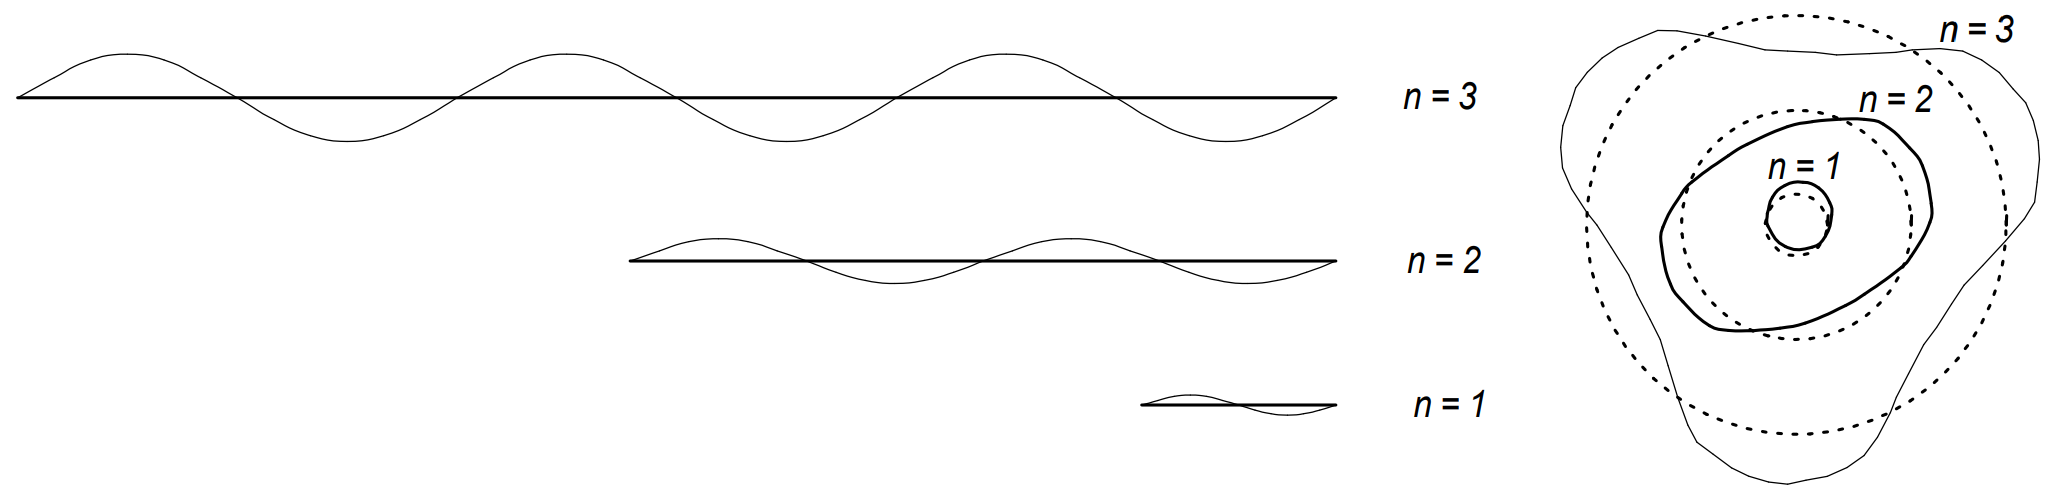
\includegraphics[width=\textwidth]{images/08_debroglie/standing-waves.png}
  \end{center}
  \caption*{\emph{Figure 2: de Broglie wavelengths for the first three Bohr orbits of
     hydrogen. In general the wavelength for the orbit of radius $a_n$ is
     $\lambda_n = 2\pi a_n/n$. (The diagram is not drawn to scale.)}}
\end{figure}



\section*{C. Packets of Matter Waves: Application to the Free Particle }

In a late work of his, reporting on his point of departure for
developing the idea of matter waves, de Broglie stresses the merely
approximate character of geometrical, or ray, optics\footnote{See note 5
  in Section A above.} and, hence, of the old, Newtonian mechanics:

\begin{quotation}
As early as 1923 I had formulated the fundamental idea that traditional
Mechanics (in both its relativistic and classically Newtonian form) was
only an approximation with the same range of validity as geometrical
Optics. From that moment I was led to realize the necessity of
constructing a new Mechanics, an undulatory Mechanics [\ldots].

In every case where Geometrical Optics is sufficient to describe the
propagation of the $\Psi$ wave {[}as the matter wave came to be
designated{]} [\ldots] the trajectories, determined by the Classical
Dynamics of a point mass [\ldots] will be simply the rays of propagation of
the $\Psi$ wave [\ldots].

And thus we arrive at one of the main ideas of the new Mechanics.
Whereas the older Mechanics attributed a rigorous character to {[}the
equations of these trajectories{]} and considered them valid everywhere,
the new Mechanics gives the leading role to the wave. It considers the
equations of the older Mechanics as approximations valid only when the
approximation of Geometrical Optics is sufficient to describe the
propagation of the wave.

Classical Dynamics thus appears to be only an approximation. It is
applicable only when the index {[}of refraction{]} $n$ relative to
the $\Psi$ wave varies only slightly in comparison with a wave-length
or, what is essentially the same thing, when the potential
$V$\footnote{{[}In the case of the orbiting electron, this would be
  the electrical potential of the electric field due to the positively
  charged hydrogen nucleus. That is what causes the trajectory of the
  electron to curve analogously to the way in which an index of
  refraction $n \propto 1/r$ would cause a light ray to curve in a
  circle. We shall see below how it is ``essentially the same
  thing.''{]}} varies slowly over the distance of a wave-length.
However, if the wave-length of the $\Psi$ wave were infinitesimally
small, the older Dynamics would be rigorously valid.\footnote{{[}L. de
  Broglie, \emph{Non-linear Wave Mechanics: A Causal Interpretation}
  (Amsterdam: Elsevier, 1960), 7, 19--20.{]}}
\end{quotation}

Thus far we have not seen how the motion of material particles as
determined by geometrical optics, that is, as being the trajectories, or
rays, determined by the matter waves, is only approximate. For, as
explained in Section B, the Bohr orbits of the electron in the hydrogen
atom appeared to be exact, not approximate. In Section B, however, it
was only claimed that the electron is localized in certain orbits;
nothing was said about its motion around an orbit. The examples
discussed in the 1923 articles did not manifest that approximate
character. Now in order to make clear that the motion of a particle is
not \emph{exactly} the motion determined by geometrical optics, we shall
imagine the motion of a free electron, such as one shot at a screen, as
in the cathode-ray tube. We ask whether there is a wave phenomenon that
moves toward the screen in roughly the same way as does the classical
electron.

To answer this question we follow de Broglie's procedure in his
dissertation,\footnote{The following account is based on his summary
  presentation in L. de Broglie, ``On the Parallelism between the
  Dynamics of a Material Particle and Geometrical Optics,'' \emph{op.\
  cit.,} 10--11.} written in 1924. There, in order to establish ``a close
connection between the propagation of the wave and the dynamics of the
associated corpuscle,''\footnote{\emph{Ibid}., 12.} he made use of a
familiar general wave phenomenon, known as a \emph{group} of waves, or a
\emph{wave packet}, which was not studied in Junior Laboratory. A wave
packet might be thought of as a wave phenomenon that concentrates its
energy in a ``burst.'' Many wave phenomena can exhibit ``burst-like''
features. For example, a vibrating string produces a steady tone, but
two strings slightly out of tune also produce ``beats,'' a regular rise
and fall in volume. Similarly, a rock dropped in a pond causes a
distinct \emph{band} of ripples to spread out, rather than a constant
undulation all across the pond.

Take a closer look at the disturbance caused by dropping a rock in a
pond. Within the band, the ripples are moving
just as a train of sine-waves would, except that each ripple
\emph{starts up} or \emph{emerges} at the trailing edge of the
band and \emph{fades out} at its leading edge. The ripples are moving
through the band, at a greater speed than the band itself, but are
noticeably present only inside the band. Consider a patch of water some
distance from the point where the rock is dropped; that patch remains
undisturbed until the band reaches it, which takes longer than the
ripples would if they moved continuously from the rock. In fact, in
water such a band moves at a speed that is only about half that at which
the ripples in it are moving. But the band is nothing but a band of
ripples. The ripples build up a distinct band, but disappear outside it.
This makes sense only if the ripples are actually a sum of component
waves which add up constructively to form the band, but add up
destructively to cancel themselves out outside the band. The band of
ripples is a moving reinforcement, or interference pattern.

Suppose, then, that a particle is accompanied not by one phase wave but
by a collection of them. It is possible that the sum of the phase waves
might produce a wave packet, a single localized region in which that sum
had an amplitude other than zero, while cancelling itself out everywhere
else. Like the band of ripples, the wave packet would move more slowly
than the individual waves within it. The particle could then be thought
of as riding along in the wave packet, as in Figure 3.


\begin{figure}[h] % Figure 3
  \begin{center}
    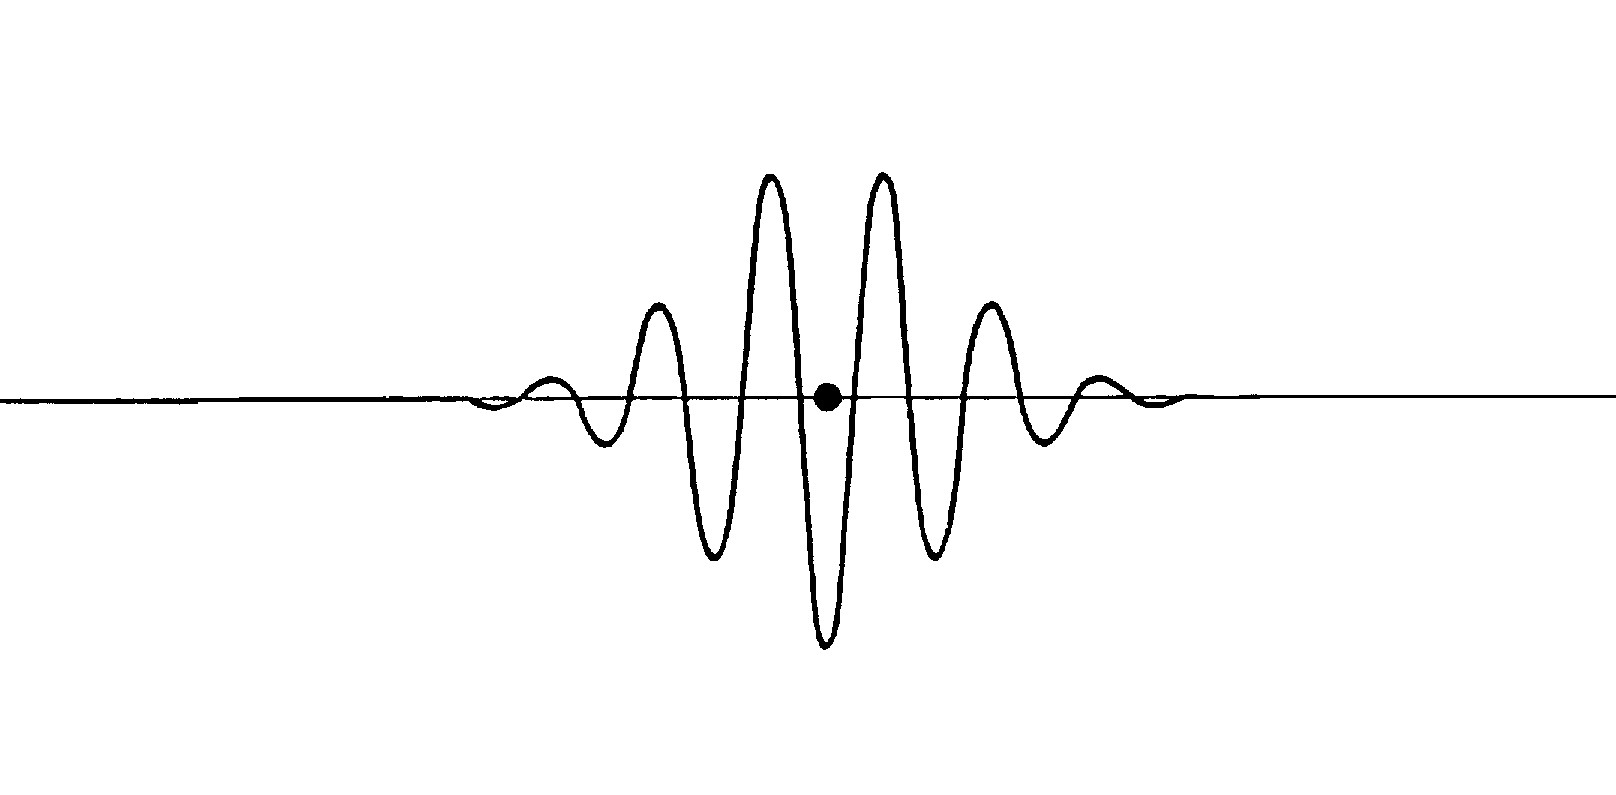
\includegraphics[width=.7\textwidth,height=.34436\textwidth]{images/08_debroglie/pilot.jpg}
  \caption*{\emph{Figure 3}}
  \end{center}
\end{figure}

The speed of a component phase wave is called the \emph{phase velocity}.
The speed of the packet is called the \emph{group velocity}. Now, the
phase velocity is determined by the two de Broglie relations for the
values for the total energy $E$ and momentum $p$ of the
particle, since they determine $\nu$~and $\lambda$,~the product of
which is the phase velocity $u$. The group velocity $g$ of the
wave packet is in turn determined by the mathematics of the addition of
wave functions; however, the particle's velocity $w$ is already
contained in the quantity $p$. The wave packet is a leading
candidate for fulfilling the role of a matter-wave phenomenon that would
move in such a way as to determine the approximate location of the
particle at any time. Hence, if it is to succeed in fulfilling that
role, de Broglie must show that $g = w$. Recall, too, that
in Section A the speeds $w$ and $u$ were assumed inversely
proportional: $wu = c^2$. As we shall see, the mathematics of
wave packets must retain this inverse proportionality between the speeds
$w$ and $u$.

Here are some examples of wave packets in various media. In a simple
wave phenomenon, a disturbance of some amplitude in a medium propagates
at a constant speed. In the simplest case from Junior Laboratory, the
medium is a rope and the disturbance is a displacement up and down of
particles along it, propagating in the one dimension of the string's
extension when we shake it up and down once. When a rock is dropped into
water, the disturbance is again an up-and-down displacement in the
medium of water, but now the propagation is in two dimensions across the
water's surface. A sound wave coming from the striking of a gong
propagates in three dimensions through the medium of air; this is
possible because the displacement of particles is forward-and-back in
the direction of propagation, longitudinal rather than transverse.

In Maxwell's theory of light, a disturbance from the flash of a signal
light is a pulse in electric and magnetic field strengths that is both
transverse and three-dimensional. The material medium, the ether,
postulated by Maxwell was, however, soon rejected as having
contradictory properties; thus the ``medium'' of light remains nothing
but a distribution of potential energy in empty space. An
electromagnetic pulse of light may be understood by analogy to the sound
wave due to the striking of a gong, but with the medium removed and the
amplitudes replaced by oscillating field strengths, transversely
directed and oriented perpendicularly to each other.

The groups of phase waves of wave mechanics take a further step away
from concreteness. They have no material medium, and their amplitudes
are simply assigned the letter $\Psi$~.~~They are groups of $\Psi$
waves in a non-physical medium, which can, however, be characterized by
an index of refraction: $n = n(x,y,z,\nu)$, as we have seen in
Section B. Hence, the medium can be expected to manifest itself by its
effect on the velocity of a wave group.

Before attempting to demonstrate what de Broglie termed the ``Theorem of
Group Velocity,'' namely, that the group velocity equals the particle
velocity: $g = w$, we shall become familiar with the
mathematics of the composition of a group of phase waves in general and
of the determination of the group velocity.

Any function of the form $f(x-ut)$ represents a
configuration that travels with velocity $u$. For consider
$f(z)$, where $z$ is measured from some point that
moves with speed $u$ in the direction of increasing $x$; so
that the graph of $f(z)$ is certainly moving with speed
$u$. But, as Figure 4 shows, $z = x-ut$.
Therefore the graph of $f(x-ut)$ also moves with
speed $u$. It is not necessarily periodic.


\begin{figure}[h] % Figure 4
  \begin{center}
    \captionsetup{width=3.4in}
    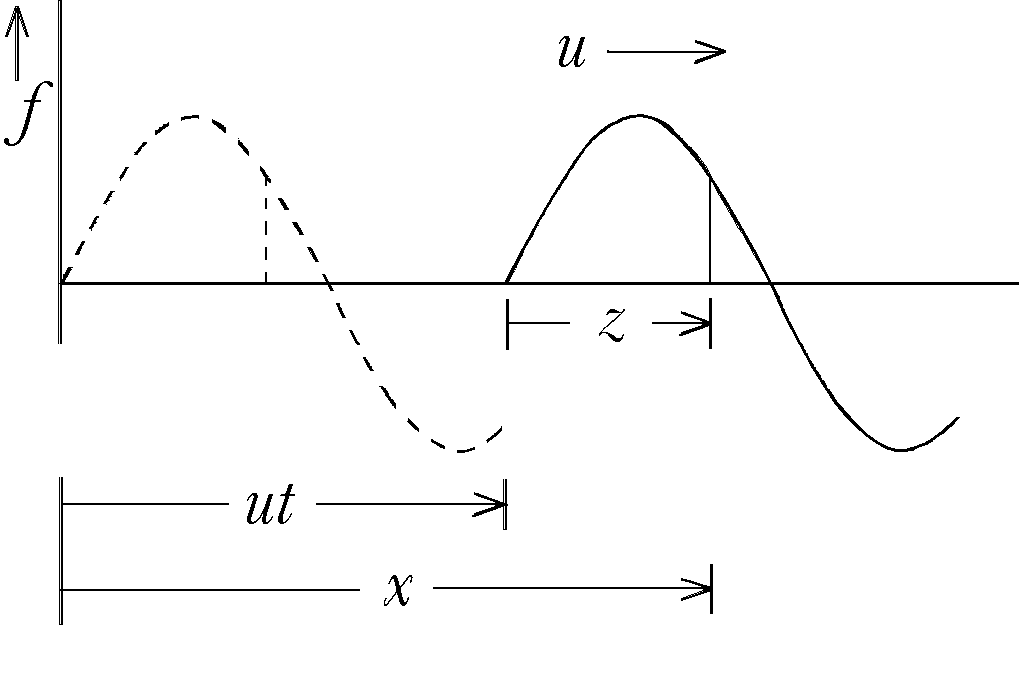
\includegraphics[width=3.4in,height=2.28in]{images/08_debroglie/image025.png}
    \caption*{\emph{Figure 4. The solid curve $f(z)$ moves with speed $u$.
    The dotted curve shows its position at some earlier moment. As the
    drawing shows, $z = x - ut$; and thus
    $f(z)$ is identical to $f(x-ut)$.}}
  \end{center}
\end{figure}

The function
\begin{equation*}
\Psi(x,t) = A \sin 2\pi k(x-ut)
\end{equation*}
not only travels with velocity $u$ as above; it, in addition, shows
periodicity at spatial intervals $\lambda$ such that $2\pi k\lambda = 2\pi$ 
which gives $\lambda = 1/k$ (this is apparent when
$t = 0$), and at time intervals $T$ such that $2\pi kuT = 2\pi$ 
from which it follows that $T = 1/ku$ (apparent
for $x = 0$). $\lambda$ is the \emph{wavelength}, and $T$ is
called the \emph{period}. The quantity \emph{k}, the inverse of
the wavelength, is called the \emph{wave number} (it is the
\emph{number} of wavelengths per unit distance). The quantity $A$
is the \emph{amplitude}, the maximum ``height'' of the wave disturbance.

When written as above, namely
\begin{equation*}
\Psi(x,t) = A \sin 2\pi k(x-ut)
\end{equation*}
the traveling wave may be said to be expressed in \emph{velocity} form,
inasmuch as it shows the velocity $u$ explicitly.

The frequency is the inverse of the period; that is, variously
expressed:
\begin{equation*}
\nu = 1/T = ku = u/\lambda .
\end{equation*}
With these substitutions, the traveling, periodic wave given above may
also be written in the form
\begin{equation*}\tag{1}
\Psi(x,t) = A \sin 2\pi(kx-\nu t)
\end{equation*}
which may be called the \emph{frequency} form; it shows the frequency
$\nu$ explicitly. Although the wave velocity is not here overtly
expressed, it will be clear from the preceding that $u = \nu\lambda = \nu/k$.

Each of de Broglie's phase waves must obey, in any one dimension,
Equation 1. To see how a wave packet is composed, let us add two waves
that differ slightly in frequency and wavelength. If
\begin{equation*}
\Psi_1  = A\sin 2\pi(kx-\nu t)\quad\text{and}\quad\Psi_2 = 
A\sin 2\pi((k+\Delta k)x - (\nu + \Delta\nu)t),
\end{equation*}
then their sum\footnote{A crucial trigonometric identity for much of
  what follows is: 
  \begin{equation*}
  \sin a + \sin b = 2 \sin\left(\frac{a+b}{2}\right)\cdot\cos\left(\frac{a-b}{2}\right) .
  \end{equation*}
  It can be derived, with some labor, from the better-known identities
  \begin{equation*}
  \sin{(a+b)} = \sin a\cos b + \cos a\sin b.
  \end{equation*}
  (and the special case in which $\sin{2a} = 2\sin{a}\cos{a}$) and
  $\cos{(a-b)} = \cos{a}\cos{b} + \sin{a}\sin{b}.$} is

\begin{equation*}
\Psi_{1+2} = 2A\cos 2\pi\left(\frac{\Delta k}{2}x - \frac{\Delta\nu}{2}t\right)
\cdot \sin 2\pi\left(\frac{k\!+\!(k\!+\!\Delta k)}{2}x - \frac{\nu\!+\!(\nu\! + \Delta\nu)}{2}t\right).
\end{equation*}

We have manipulated this equation algebraically to bring out its formal
resemblance to Equation 1. The sine factor here corresponds to the sine
factor in Equation 1, but here the coefficient of $x$ is the
average of $k$ and $k\! + \Delta k$, while the coefficient of
$t$ is the average of $\nu$ and $\nu\! + \Delta\nu$; thus the
sine factor represents a wave whose wave number is the average of the
two component wave numbers and whose frequency is the average of the two
component frequencies.

The amplitude $A$ in Equation 1 corresponds here to the whole
factor 
%
\begin{equation*}
2A\cos 2\pi\left(\frac{\Delta k}{2}x - \frac{\Delta\nu}{2}t\right) , 
\end{equation*}
%
which thus plays the role of a \emph{variable} amplitude, the
\emph{envelope}. The maximum value of the envelope is $2A$, which
is twice the amplitude $A$ of either component. This indicates that
the sum of the two waves attains a maximum wherever two crests or two
troughs of the component waves add up. Since the envelope also involves
a cosine term, and since the cosine exhibits the same wavelike shape as
the sine, the envelope can itself be viewed as a wave: its wave number
will be half the difference of the component wave numbers, and its
frequency will be half the difference of the component frequencies. The
compound wave formed by adding two components thus seems to be acting
like a wave in two ways at once (see Figure 5).

\begin{figure}[h] % Figure 5
  \begin{center}
    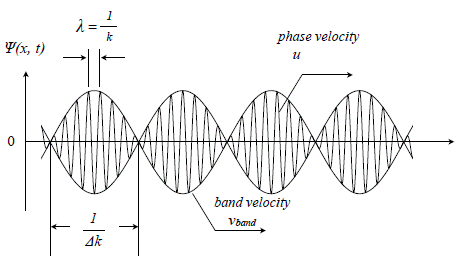
\includegraphics[width=4.90625in,height=2.85417in]{images/08_debroglie/image036.png}
    \caption*{\emph{Figure 5}}
  \end{center}
\end{figure}

In the figure the dense inner line graphs the sine factor. Its wavelength is
labeled as $\lambda = 1/k$. This is approximately true: since
$\Delta\lambda$ was chosen to be small, the wavelength of $\Psi_2$ differs
little from $\lambda$, the wavelength of $\Psi_1$, and the average of
the two wavelengths differs from it even less. The speed of propagation
of the inner-line wave is the phase velocity $u$. The more relaxed
outline graphs the cosine factor, the envelope surrounding the
higher-frequency wave. The graph also shows the meaning of the two factors in
the expression for $\Psi_{1+2}$: the compound wave is a wave within a
wave. Thus two component waves of slightly different frequencies and
wavelengths will combine to form an interference pattern consisting of a
succession of bands enveloping or containing a wave of shorter
wavelength and higher frequency.

This is not quite where we want to be, since the envelope is an endless
string of adjacent bands rather than a single isolated wave packet.
Nevertheless, it permits us to form a simple equation deriving the
velocity of any band in the envelope---which could be viewed in
isolation as a group formed of two component phase waves---from the
properties of its two component phase waves. Since the speed of any wave
in general is the product of its wavelength and frequency, and since we
can read these values \emph{for any band} from the coefficients in the
cosine factor, the band velocity, $u_{\text{band}}$, may be
expressed as

\begin{equation*}\tag{2}
u_{band} = (\text{wavelength})\!\times\!(\text{frequency}) = \frac{2}{\Delta k}\frac{\Delta\nu}{2} = 
\frac{\Delta\nu}{\Delta k}
\end{equation*}

Figure 6 shows how the two component waves build up the compound
envelope and its bands. The two components are shown in a ratio of
wavelengths of 9~:~8. At (a), crests of the longer and the shorter wave
coincide to produce a maximum in their sum. Then at (b), after 4 full
cycles of the longer and 4-$\frac{1}{2}$ of the shorter, a crest of the longer
component coincides with a trough of the shorter one, producing a node
in the compound wave. At (c) both components display crests again,
producing a maximum in their sum once more. Each repetition of the same
interval brings the two components back out of phase 180$^{\circ}$ at a node, or
back in phase at a common crest.

\begin{figure}[h] % Figure 6
  \begin{center}
    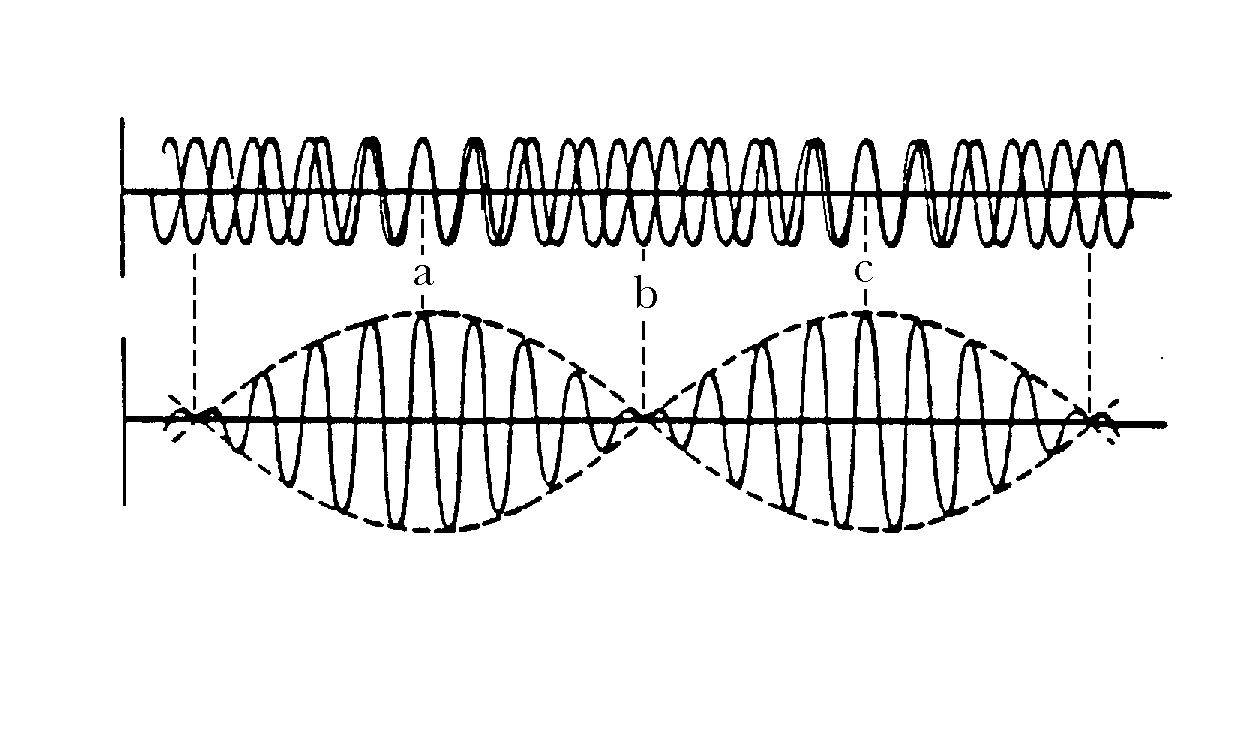
\includegraphics[width=4.18333in,height=2.51667in]{images/08_debroglie/image039.png}
    \caption*{\emph{Figure 6}}
  \end{center}
\end{figure}

The pattern in Figure 6 must continue indefinitely. But what happens if
we add a third component wave with a wavelength and frequency between
those of the first two components? If we add a fourth? A fifth?
Infinitely many? Figure 7 may suffice to answer these questions in a
general way. It shows a sum of six component waves. The envelope will
clearly have its maximum amplitude at every point where all the
components reach a crest together, and these points will also be the
centers of the bands. But each additional component wave increases the
distance between the centers of bands. To see why, look once more at
Figure 6.

\begin{figure}[h] % Figure 7
  \begin{center}
    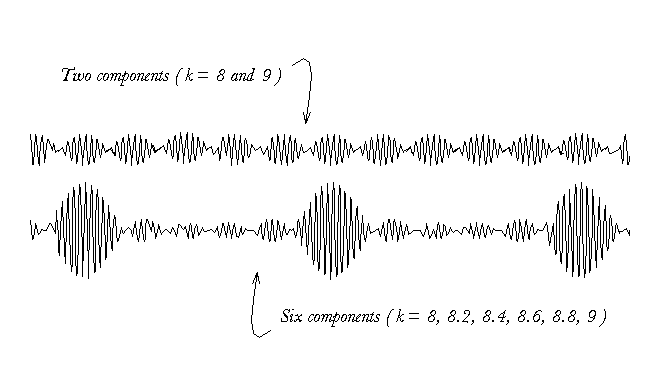
\includegraphics[width=4.35334in,height=2.52in]{images/08_debroglie/image041.png}
    \caption*{\emph{Figure 7. Six component waves of the indicated wave numbers, two of
     which are shown on top, are added to produce more widely separated bands
     of greater amplitude.}}
  \end{center}
\end{figure}

There, a third component with a wavelength halfway between the two shown
would cycle 8-$\frac{1}{2}$ times between (a) and (c). If the third component were in
phase with the first two at (a), then it would be out of phase with them
at (c) and would subtract its amplitude from their sum. With proper
choice of amplitudes, every second maximum could be nearly canceled; the
distance between adjacent common maxima of all three components would
then be double the distance for the first two alone. So by adding ever
more intermediate component waves---canceling out every third, fourth,
fifth maximum, and so on---we can eventually move the centers of
adjacent bands as far apart as we please.

Does each band stretch to fill the longer interval? Figure 7 suggests
that it does not, but that instead the envelope cycles up and down near
the baseline between bands that themselves remain narrow. As more and
more intermediate component waves are added and the common crests become
fewer and farther between, there are also more and more opportunities
for every component at every spot in between to have an amplitude nearly
equal and opposite to that of some other component; so that the
amplitude of the envelope will fall off rapidly on both sides of each
maximum, and tend everywhere else toward zero.

This suggests, and it can in fact be proved, that if we added a
countable infinity of suitably selected\footnote{The infinity of values
  of $k$ between 8 and 9 must be everywhere dense on the interval
  {[}8,9{]}; that is, given any one of them, it must be impossible to
  find an interval containing it that does not also contain
  another---and, in fact, an infinity---of the selected points in its
  interior.} intermediate component waves while focusing our attention
on a single band, the other bands would be removed to an infinite
distance, leaving the single wave packet of Figure 3. This claim is
analogous to that of Daniel Bernoulli that ``all sonorous bodies contain
potentially an infinity of sounds, and an infinity of corresponding ways
of making their regular vibrations'' (\emph{Mechanics}, 201).\footnote{In
  fact, given any ``reasonable'' finite curve represented by a function
  $f(x)$ on an interval (0,$L$), and such that $f(0) = 0
  = f(L)$, we may determine the constants
  $A_n$ such that the curve is represented by an
  infinite sum of sinusoidal curves: 
  \begin{equation*}
  f(x) = \sum_{n=1}^{\infty}A_n \sin (n\pi x/L). 
  \end{equation*}
  We could
  imagine $f(x)$ as representing a snapshot of the top half
  of a wave packet at any time. Similarly, if $g(x,t)$ is a
  ``reasonable'' function, which here represents the forward motion of
  the top half of a wave packet, then it is possible to determine the
  constants $B_n$ such that $g$ may be
  represented as a sum of an infinite number of standing waves (compare
  \emph{Mechanics}, 204):
  \begin{equation*}
  g(x,t) = \sum_{n=1}^{\infty} B_n \sin (n\pi x/L) \cos (2\pi\nu t).
  \end{equation*}
  }

To keep the amplitude of the packet finite, while adding infinitely many
increments to it, we could, for example, let the amplitudes of the
outermost components each be 1, that of the central one 1/2, those of
the two halfway between the central and outermost ones 1/8, etc.---the
amplitude of the packet would then be
\begin{equation*}
2 + 2^0\cdot(1/2)^1 + 2^1\cdot(1/2)^3 + 2^2\cdot(1/2)^5 \ldots = 3.
\end{equation*}
In this way we could construct an envelope that is a single wave packet rather
than an infinite series of bands. The same reasoning that led to Equation 2 for
the bands in an envelope now applies to an envelope of only one band.
Hence, we have for the velocity of the packet, the group velocity:

\begin{equation*}\tag{3}
g = \frac{\Delta\nu}{\Delta k}.
\end{equation*}

The exact way in which the group would move depends on its index of
refraction. Even though this medium in which the $\Psi$ waves move is
unknown, it can be characterized in one way by its effect on the speed
of the waves. For just as in empty space (index of refraction constant:
$n$ = 1) all electromagnetic waves, whatever their frequency, move
at the same speed $c$, so, if the index of refraction were the same
for $\Psi$ waves of different frequencies, then every component phase
wave in a group would have the same speed $u$. Under this
condition, the phase velocity would also have to be equal to this
constant $u$. What would the group velocity then be? Since
\begin{equation*}
k = \frac{1}{\lambda} = \frac{\nu}{u},
\end{equation*}
therefore, where $u$ is a constant,
\begin{equation*}
g = \frac{\Delta\nu}{\Delta k} = \frac{\Delta\nu}{\Delta(\nu/u)} =
\frac{\Delta\nu}{\Delta\nu/u} = u\frac{\Delta\nu}{\Delta\nu} = u,
\end{equation*}
and the wave packet would move with the same speed as the compound phase
waves within it. But we want the packet to keep pace with the particle
at speed $w$, which must be inversely proportional to $u$.

Already in Section B, in order to derive the Bohr orbits from matter
waves, we saw that de Broglie had supposed that the index of refraction
for them depended on both location and the frequency of the waves:
$n = n(x,y,z,\nu)$, that they moved in a dispersive medium.
Now we shall prove that the two de Broglie relations $E =h\nu$ and 
$p = h/\lambda$ imply that the $\Psi$ waves
\emph{are} subject to dispersion. For,
\begin{equation*}
u = \nu\lambda = \frac{E}{h}\frac{h}{p} = \frac{E}{p} = \frac{h\nu}{p}.
\end{equation*}
And
\begin{equation*}
p = mw = \sqrt{m^2w^2} = \sqrt{2m\cdot\frac{mw^2}{2}} = \sqrt{2m(E-V)}
= \sqrt{2m(h\nu - V)},
\end{equation*}
where the total energy of the particle minus its potential energy $(E - V)$ has
been substituted for its kinetic energy. Substitution of the above
expression for $p$ into the equation for $u$ gives
\begin{equation*}\tag{4}
u = \frac{h\nu}{\sqrt{2m(h\nu -V)}}.\footnote{$V$ here is potential energy. If $E$ is substituted
  for $h\nu$ in Eq. 4, the resulting equation,
  \begin{equation*}
  u = \frac{E}{\sqrt{2m(E-V)}}
  \end{equation*}
  is identical to Schrödinger's Equation 8, in Chapter 10. There he
  develops a differential equation for the $\Psi$ waves like that for
  the vibrating string. Then by assuming that his Equation 8 is a
  solution to this differential equation, he is able to determine a
  time-independent differential equation for the part, designated
  ``$\psi$,'' of the $\Psi$-waves that represents a standing wave.}
\end{equation*}
Now, since $V=V(x,y,z)$, therefore, by Equation 4,
the speeds, $u$, of the matter waves depend on their location and
on their frequency, $u = u(x,y,z,\nu)$. Since
the index of refraction is inversely proportional to the speed of the
waves (see note 13 above), this implies that $n = n(x,y,z,\nu)$ and that 
the matter waves do move in a dispersive
medium, as de Broglie had supposed. Just as the index of refraction of a
glass prism disperses light waves of different frequencies, so the
dependence of the wave-speed $u$ on the potential $V$ and on
the frequency of the waves is responsible for the dispersion of the
$\Psi$ waves.

In this case the group velocity, $g$, will \emph{not} turn out to
be equal to the velocity, $u$, of the component waves as happened
above when we had supposed an index of refraction that was independent
of the frequency. Instead the phase waves will ripple through the wave
packet, leaving it behind. Recall that according to Equation 3 the wave
packet will move with speed, $g = \Delta\nu/\Delta k$. Now, since
$k = 1/\lambda = \nu/u$, therefore,
$\nu = ku$, so that $\nu$ is a function of $k$.
Therefore, $\nu$~may be differentiated with respect to $k$, and
as $\Delta k$ tends toward zero, $\Delta\nu/\Delta k$ will approach the
derivative of $\nu$~with respect to $k$.\footnote{Although the
  domain of definition of the function $\nu(k)$ is not a
  continuous interval, the fact that it is a countably infinite,
  everywhere dense subset of an interval allows its derivative to be
  defined in the same way as was done in Junior Mathematics.

  When there are only \emph{two} components differing by $\Delta\nu$ and
  $\Delta k$ the expression $g = \Delta\nu/\Delta k$ is exact. When
  there is an infinity of component waves, the expression for group
  velocity is $g = d\nu/dk$, as the next equation states. This
  expression, too, is exact.

  Like any derivative $d\nu/dk$ must be evaluated at individual
  values of the independent variable. The resulting value for $g$
  will depend on whatever value is specified for the wave number
  $k$. Then, inasmuch as the wave packet comprises a \emph{range}
  for $\lambda$ and therefore for $k$, the packet may exhibit a
  corresponding \emph{range} of velocities. This is the result not of
  approximation but of heterogeneity: we cannot get a more sharply
  defined velocity for the packet as a whole by any limiting procedure.}
This yields
\begin{equation*}\tag{5}
g = \frac{d\nu}{dk} ,
\end{equation*}
which, de Broglie specifies, is to be evaluated at a value of $k$
such that $\nu = E/h$ (he conceives of this as the
central frequency of the component waves).

This group velocity, $g$, is related to the particle velocity,
$w$, through the de Broglie relation $\lambda = h/p$
or $k = p/h$. Here $k$ is a function of
$p$, the momentum of the particle, and, clearly, $dk/dp=1/h$.
Taking Equation (5) and multiplying equals by equals gives
\begin{equation*}
g\frac{1}{h} = \frac{d\nu}{dk}\frac{1}{h} = \frac{d\nu}{dk}\frac{dk}{dp}.
\end{equation*}
Then by the Chain Rule,
\begin{equation*}
g\frac{1}{h} = \frac{d\nu}{dp}.
\end{equation*}
Multiplying both sides by the constant $h$,
\begin{equation*}
g = h\frac{d\nu}{dp} = \frac{d(h\nu)}{dp} = \frac{dE}{dp}.
\end{equation*}
This equation expresses the group velocity of the wave packet in terms
of $E$ and $p$, the total energy and the momentum,
respectively, of the particle.

At this point we can prove de Broglie's Theorem of Group
Velocity:\footnote{L. de Broglie, \emph{Non-linear Wave Mechanics: A
  Causal Interpretation} (Amsterdam: Elsevier, 1960), 24.}
\emph{If a group of $\Psi$ waves is associated with the motion of a particle,
and if the central frequency of the group corresponds to the total
energy of the particle, then the group-velocity will be equal to the
particle's velocity.} For we have just seen that $g = dE/dp$. But the total 
energy equals the kinetic energy plus the
potential energy. Further, $p = mw$, so that
$p^2 = m^2w^2$ and thus the kinetic
energy $K$ can be written as $p^2/2m$;
substituting gives
\begin{equation*}
\frac{dE}{dp} = \frac{d}{dp}\left(\frac{p^2}{2m} + V\right).
\end{equation*}
Furthermore, the potential energy $V$ is a function of the spatial
coordinates only, so it acts like a constant when one differentiates
with respect to $p$; and $\frac{1}{2}m$ is simply a constant. Thus,
\begin{equation*}
\frac{d}{dp}\left(\frac{p^2}{2m}+V\right) = \frac{1}{2m}\left(\frac{d}{dp}(p^2)+0\right) = \frac{1}{2m}2p.
\end{equation*}
And in turn
\begin{equation*}
\frac{1}{2m}2p = \frac{mw}{m} = w ;
\end{equation*}
And, therefore,
\begin{equation*}
g = \frac{dE}{dp} = w.
\end{equation*}
When $E$ equals the total energy of a particle, and the central
frequency of the group corresponding to it equals $E/h$, then the
group velocity equals the velocity of the particle. Q.E.D.

Thus, in a dispersive medium the wave packet travels with the same speed
as the particle and transports the particle's energy---simply as a
result of the laws of wave propagation. But this rose has a thorn. The
very fact of dispersion that allows the wave packet to form also forces
it to disperse; the leading edge of the packet will always be moving at
a greater speed than its trailing edge.\footnote{It can be shown that
  (as one might expect) the leading edge will move with approximately
  the greatest velocity in the range mentioned in note 31 above, and the
  trailing edge with approximately the least. We cannot go into the
  details.} The wave packet can supply everything that was classically
attributed to the Newtonian particle except permanence of location.

\section*{D. The Interpretation of Matter Waves}

So far matter waves have been presented as guiding material particles.
Whereas at first de Broglie had viewed the matter wave properties of
wavelength and frequency as \emph{due to} the material particle's
momentum and energy, respectively, in his exposition in English of the
ideas he developed for his dissertation, he proposed that matter waves
are \emph{responsible for} the dynamical properties of material
particles:

\begin{quote}
I shall adopt a point of view slightly different from those which I have
developed up to now, \emph{for I shall take the laws of wave propagation
as fundamental, and seek to deduce from them, as consequences which are
valid in certain cases only, the laws of the dynamics of a
particle.}\footnote{{[}L.\ de Broglie, ``On the Parallelism between the
  Dynamics of a Material Particle and Geometrical Optics,'' \emph{op.\ 
  cit.}, 11--12.{]}}
\end{quote}

From this point of view, the particle would not only have wave
properties; every property of the particle would be given to it by its
accompanying wave.

DeBroglie was hardly the only physicist to wonder about the physical
interpretation that should be given to the mathematical formalism of
wave mechanics. As we will see in subsequent chapters, different
thinkers have produced different ways to think about the apparent
paradoxes that arise from trying to find common ground between the
formal mathematics that applies to particles and the formal mathematics
that applies to waves. And there are many more attempts than the ones we
will consider.

The question of how best to understand matter waves is still an open one
today.


\section*{Examples and Exercises with Matter Waves}

1. If every particle is accompanied by a phase wave, why are wave
effects not always evident? Consider Rutherford's experiment: a beam of
alpha particles passes through gold foil, which is a lattice of
regularly spaced atoms, with gaps between nuclei on the order of
$10^{-8}$ cm.

Since the alpha-particle is a charged helium atom, its mass will be four
times that of the hydrogen atom. At the very end of Chapter III we found
the mass of the hydrogen atom to be $1.674\!\times\!10^{-24}$ gm;
thus the alpha particle has mass $m = 6.696\!\times\!10^{-24}$ gm. And in 
Chapter IV Rutherford cites the
velocity of the alpha particle as $v = 2.09\!\times\!10^{9}$ cm/sec. Then 
the wavelength associated with these
alpha particles must be, by de Broglie's relation,
\begin{equation*}
\lambda = \frac{h}{p} = \frac{h}{mv} = 
\frac{6.625\!\times\!10^{-27}}{6.696\!\times\!10^{-24}\cdot2.09\!\times\!10^9}
= 4.73\!\times\!10^{-13}\, \text{cm}.
\end{equation*}
Thus the phase wave associated with the alpha particle has a wavelength
some 100,000 times smaller than the $10^{-8}$ cm ``slit''
through which it must pass between the gold atoms. This would be
comparable to a beam of yellow light, wavelength $5900\!\times\!10^{-8}$ cm, passing
through a slit 5.9 cm wide---for the 100,000:1 ratio is the same in both
cases. As we would not expect detectable diffraction in the optical
case, neither would discernible diffraction effects be expected in the
scattering of alpha-particles by gold foil.\footnote{For diffraction of
  light of wavelength $\lambda$ by a single slit of width $d$, the
  maximum separation of interference bands will be given by the formula
  $\sin{\theta} = \lambda/d$ (see Appendix I below). With
  $\lambda/d$ approximately equal to 1/100,000, the angular
  separation $\theta$ will only be about .0005$^{\circ}$.}

2. What is the wavelength associated with a 200g baseball traveling at
4000cm/sec (about 89.5 mph), in comparison with a 100-cm-wide doorway?
In this case, $\sin{\theta}$is on the order of $10^{-34}$,
and the first bands of the interference pattern are separated from the
center by about $10^{-33}$ (one millionth to more than the
fifth power!) degree. The matter waves of perceptible bodies produce no
perceptible effects. If one angstrom ($10^{-8}$ cm) is the
smallest slit-width available, then even something as small as an alpha
particle would have to be moving impossibly slowly to interact
detectably with the opening. On the other hand, the very small mass of
the electron makes it a promising candidate to have a discernible
wavelength.

3. Calculate the wavelength of the phase wave of the electrons in
Thomson's cathode ray experiment, for which Thomson in Chapter II
tabulated a speed of $2.8\!\times\!10^{9}$ cm/sec.

Using the values already cited, we have
\begin{equation*}
\lambda = \frac{h}{p} = \frac{h}{mv} = 
\frac{6.625\!\times\!10^{-27}}{.910\!\times\!10^{-27}\cdot2.8\!\times\!10^9}
=2.6\!\times\!10^{-9}\, \text{cm}.
\end{equation*}
Calculate the angular separation of the first bright bands produced by
passing the electron beam through a crystal lattice of atoms spaced at
intervals of 5 angstroms $(5\!\times\!10^{-8} \text{cm})$.

We shall have
\begin{equation*}
\sin{\theta}=\frac{\lambda}{d}=\frac{2.6\!\times\!10^{-9}}{5\!\times\!10^{-8}}
= .052
\end{equation*}
which gives an angular separation of nearly 3 degrees. Diffraction
effects of this size will certainly be detectable---if one knows one is
looking for them!
